\documentclass{article}

\usepackage{graphicx}

\pagestyle{headings}

\title{TEST REPORT}
\author{WANG Chen, 2015213086, wangchen@bupt.edu.cn}
\date{\today}

\begin{document}

\maketitle

\tableofcontents

\newpage
\section{INTRODUCTION}

This is a test report of simple shell program named msh.
The shell program is a course assignment in \emph{Advanced Programming in the UNIX Environment}.
It will make us have a deeper understanding in UNIX C programming, after we finish this program.
This document is contains verifications of meeting requirements in requirement documents.

\newpage
\section{REQUIREMENTS \& FUNCTIONS}

\subsection{Command Prompt}

\subsubsection{Description}

The program is executed from the console and a command prompt is displayed when it is started. For example, "\verb|->|". Users can change the command prompt by assigning values to specific environment variables.

\subsubsection{Verification}

\begin{figure}[h]
\centering
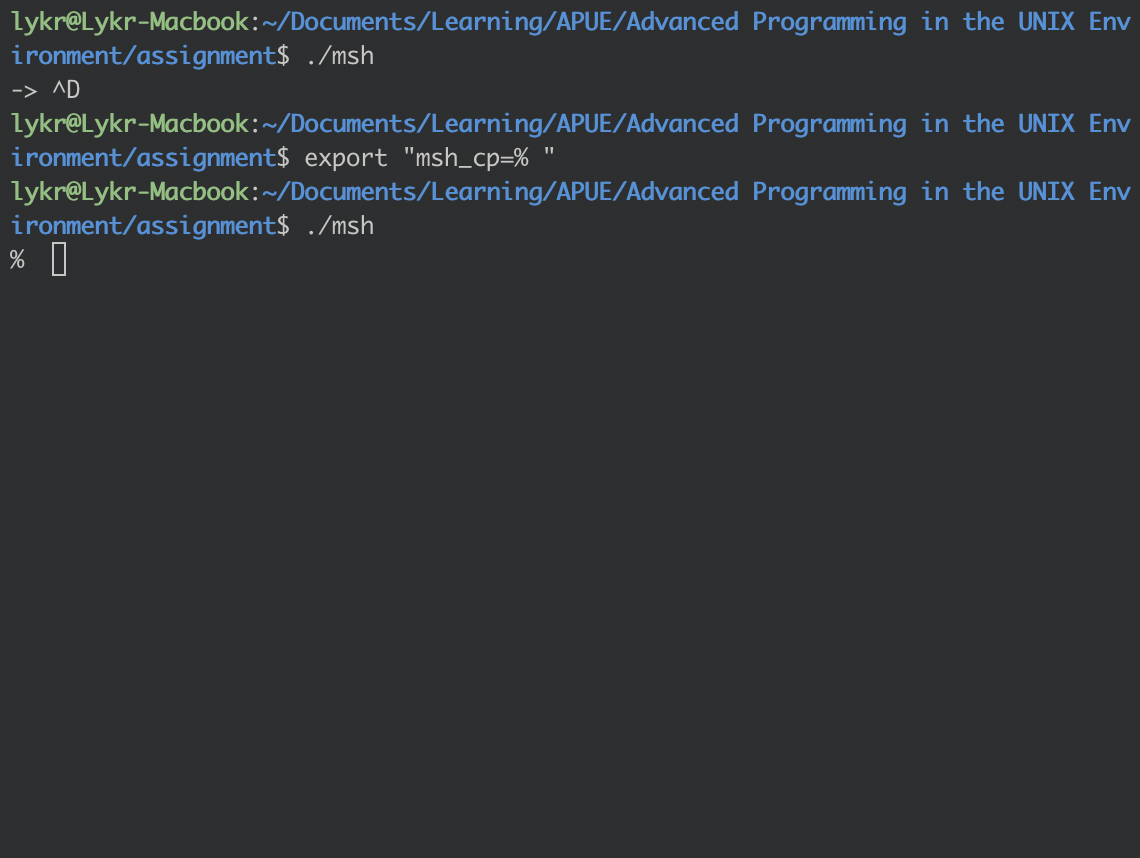
\includegraphics[scale=0.5]{fig/v1-1.png}
\caption{Run msh and display command prompt}
\end{figure}

\newpage
\subsection{Close Program}

\subsubsection{Description}

This program can be shut down normally by a special command or key combination.

\subsubsection{Verification}

\begin{figure}[h]
\centering
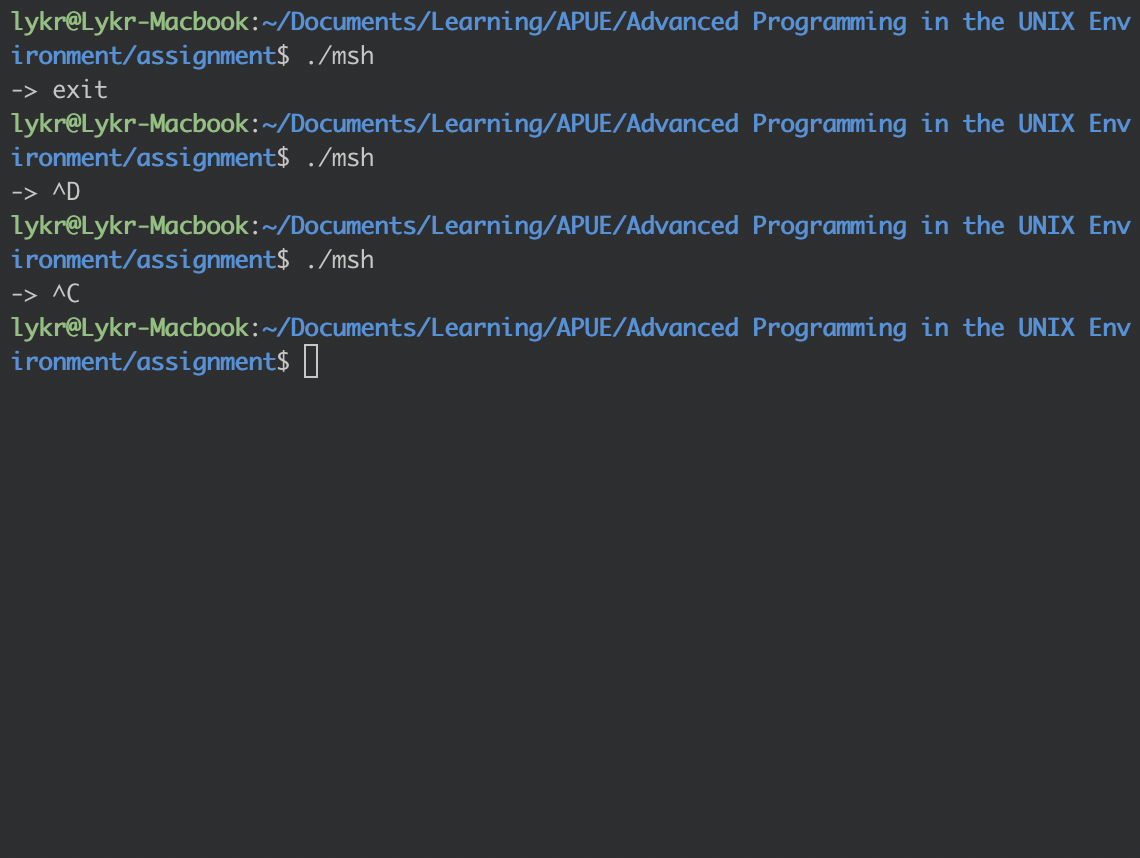
\includegraphics[scale=0.5]{fig/v2-1.png}
\caption{Close program by command or key combination}
\end{figure}

\newpage
\subsection{Runs in Background}

\subsubsection{Description}

Provide background operation mechanism. Tasks submitted by users can be made to run in the background by some instructions, such as: \verb|-> bg job1 <CR>| which will make \verb|job1| run in the background and return a new prompt to the user immediately.

\subsubsection{Verification}

\begin{figure}[h]
\centering
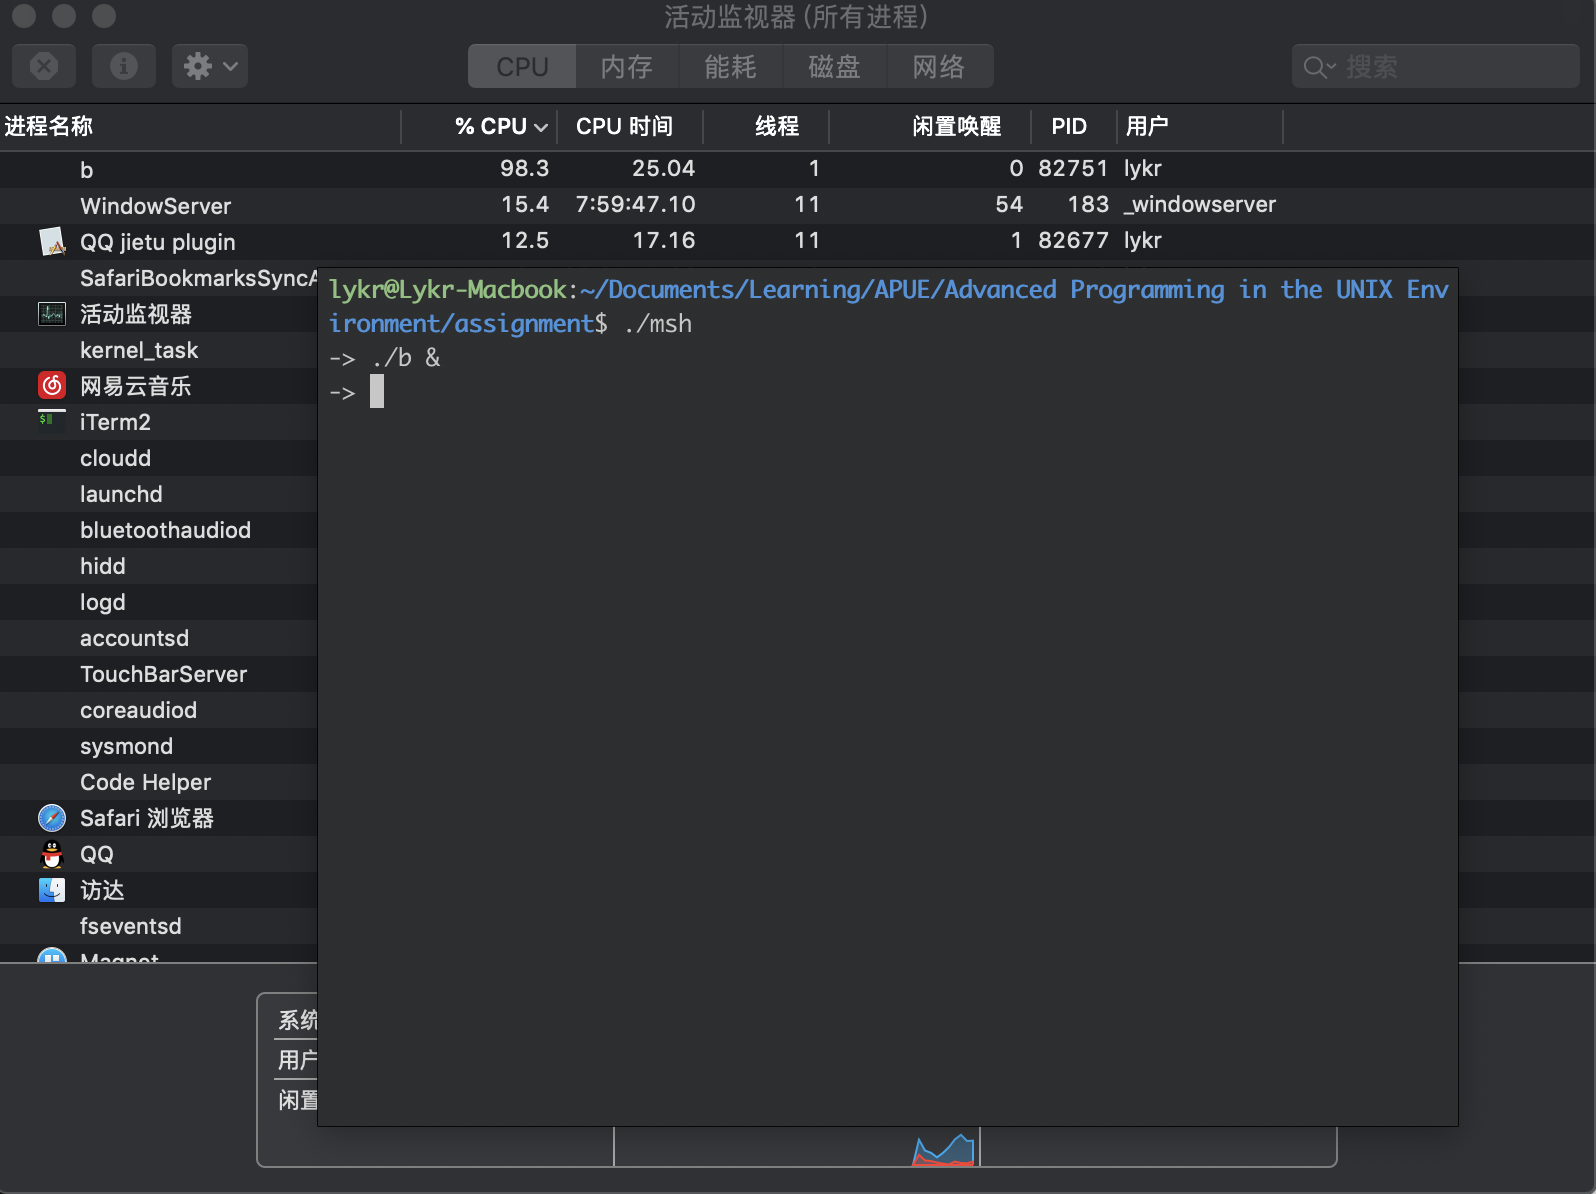
\includegraphics[scale=0.4]{fig/v3-1.png}
\caption{Program 'b' run in background and a new command prompt is presented}
\end{figure}

\newpage
\subsection{Output \& Input Redirection}

\subsubsection{Description}

Write all output of task to a file by specifying file names instead of sending them to standard output.
By specifying the file name, the task can obtain the required data from the corresponding file, rather than from the standard input.

\subsubsection{Verification}

\begin{figure}[h]
\centering
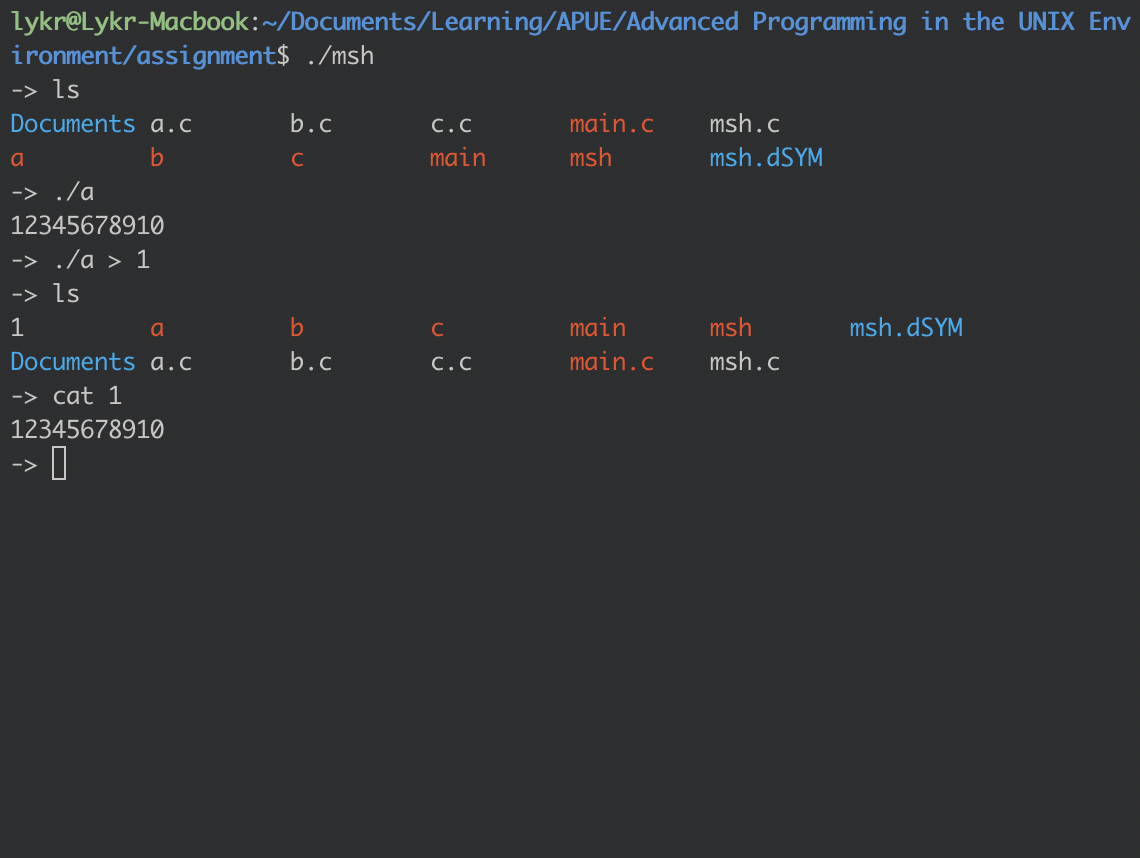
\includegraphics[scale=0.5]{fig/v4-1.png}
\caption{Output redirection}
\end{figure}

\newpage
\begin{figure}[h]
\centering
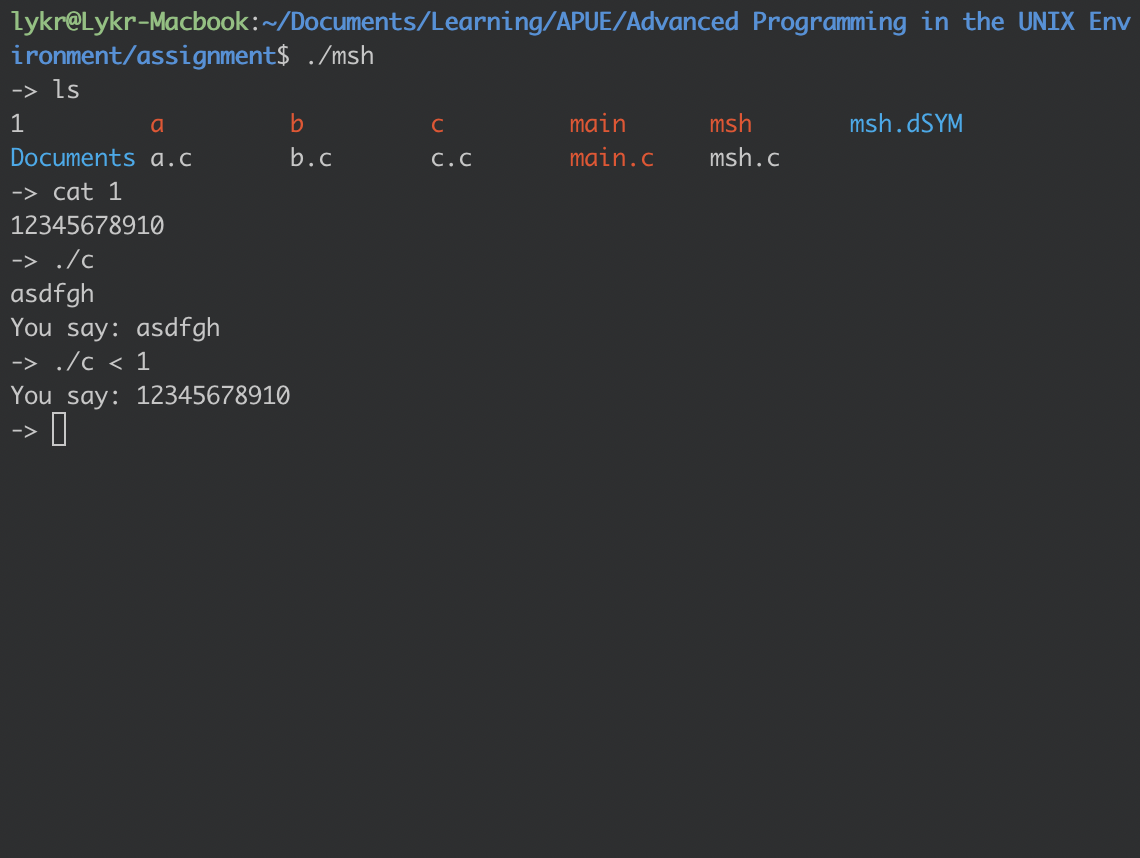
\includegraphics[scale=0.4]{fig/v4-2.png}
\caption{Input redirection}
\end{figure}

\begin{figure}[h]
\centering
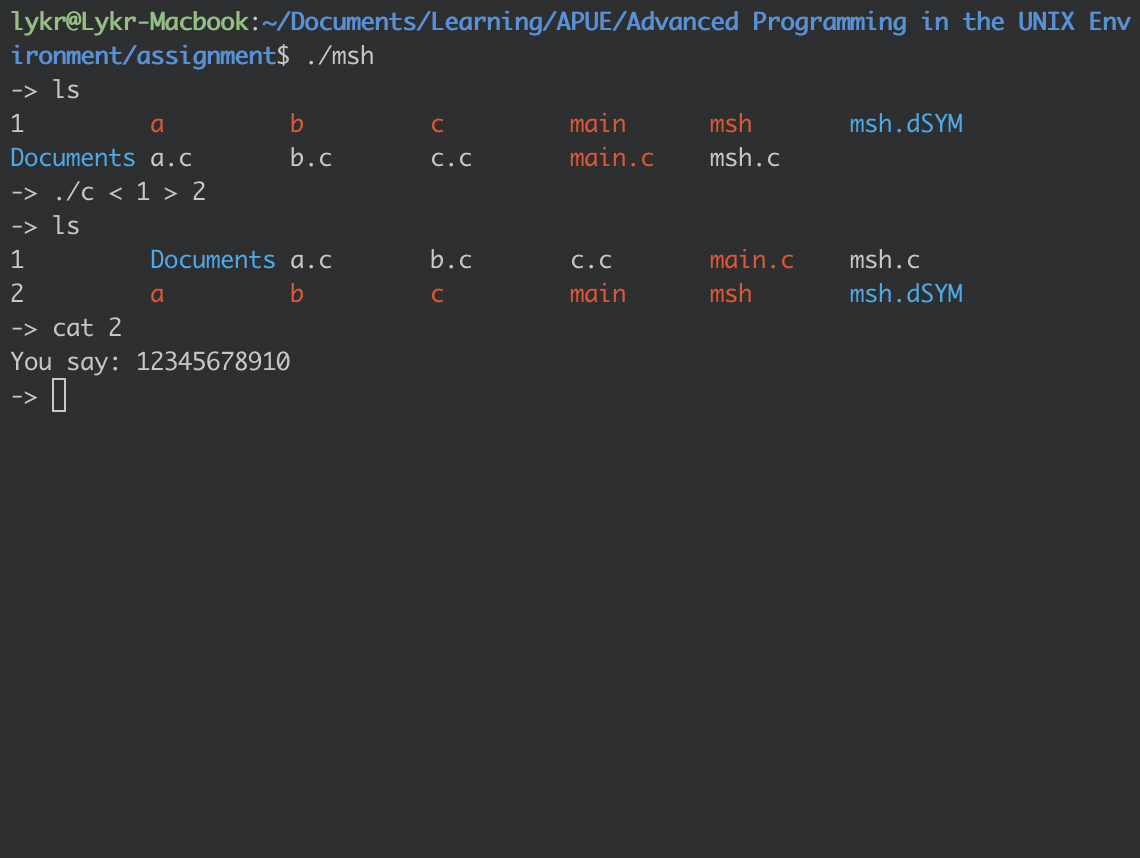
\includegraphics[scale=0.4]{fig/v4-3.png}
\caption{Input \& Output redirection}
\end{figure}

\newpage
\subsection{Other Command}

\subsubsection{Description}

The shell can execute some command like \verb|cd|, \verb|ls|, \verb|mkdir|, \verb|rm| and so on.

\subsubsection{Verification}

\begin{figure}[h]
\centering
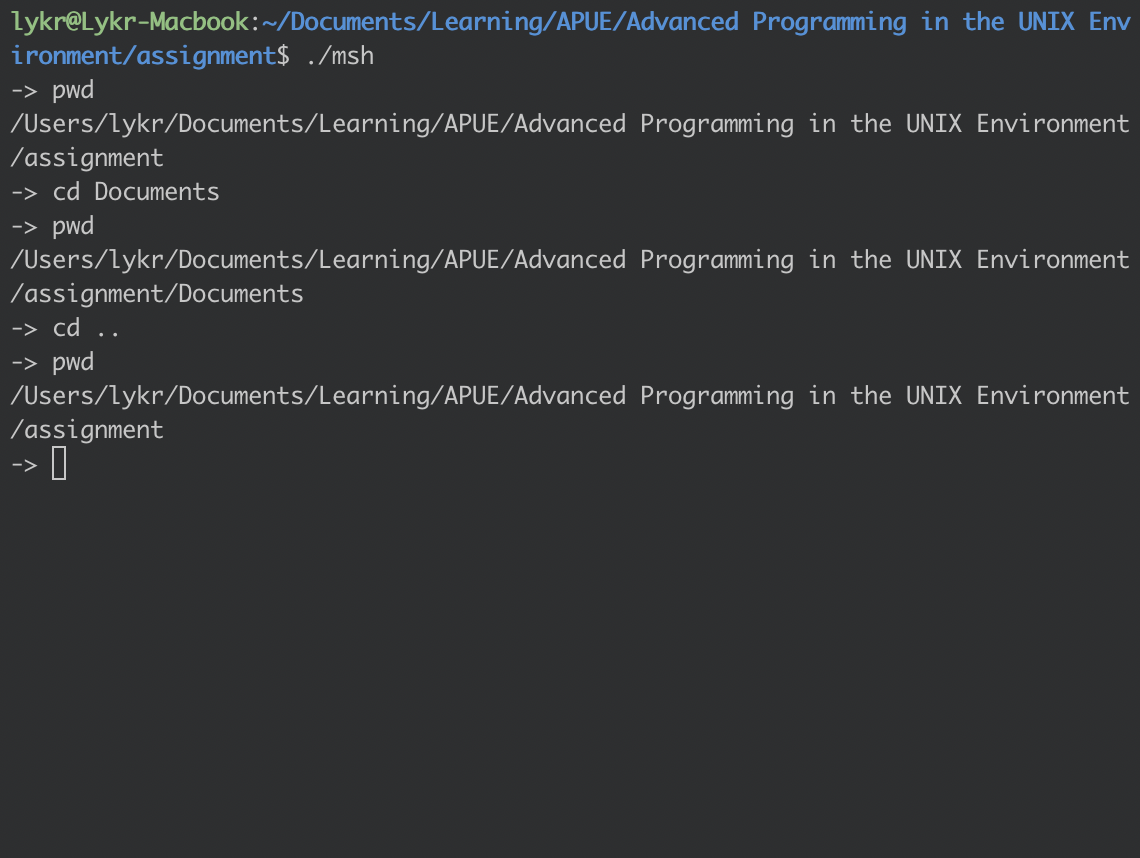
\includegraphics[scale=0.4]{fig/v5-1.png}
\caption{Command `cd'}
\end{figure}

\begin{figure}[h]
\centering
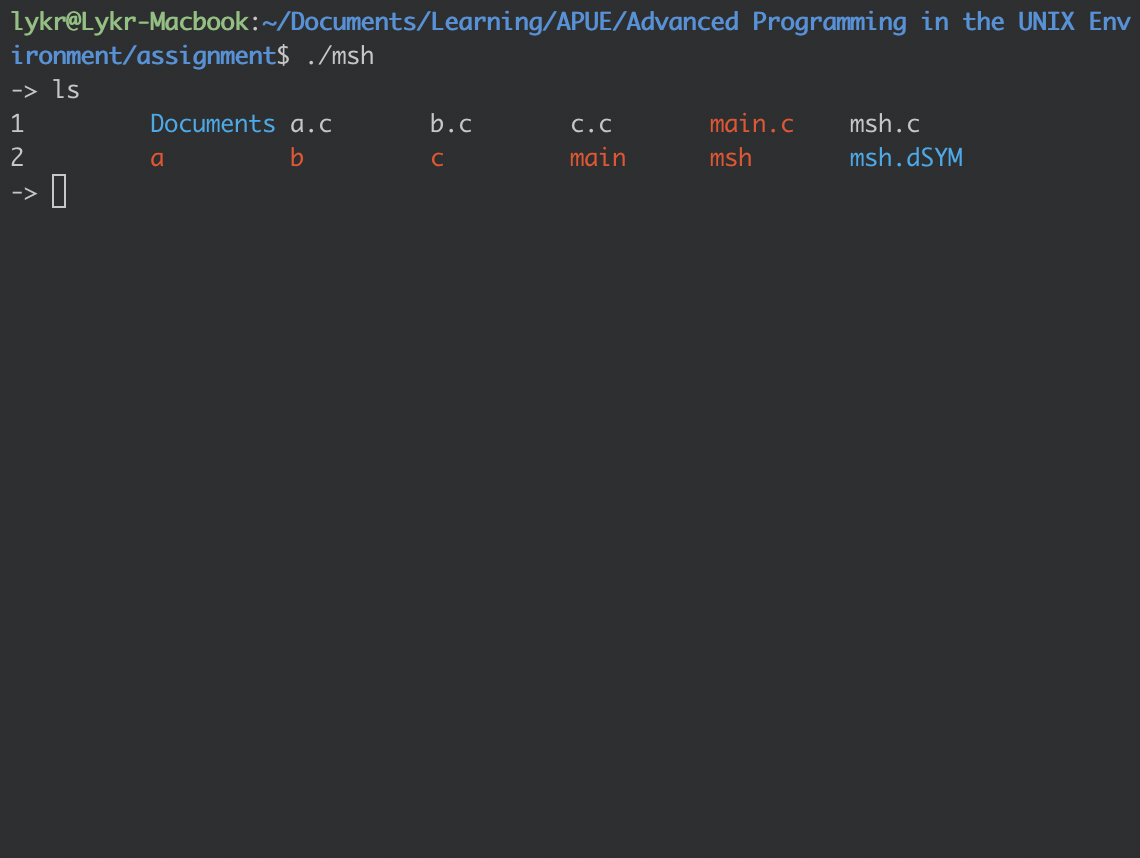
\includegraphics[scale=0.4]{fig/v5-2.png}
\caption{Command `ls'}
\end{figure}

\newpage
\begin{figure}[h]
\centering
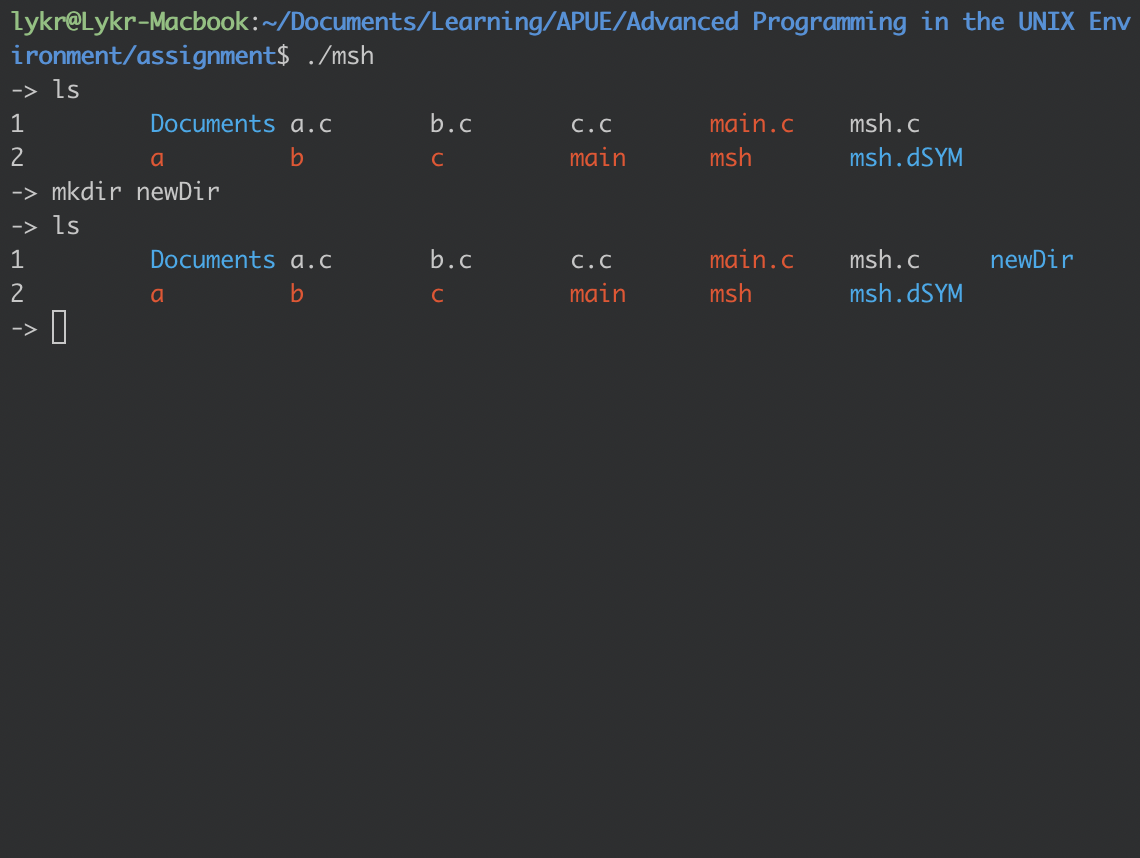
\includegraphics[scale=0.4]{fig/v5-3.png}
\caption{Command `mkdir'}
\end{figure}

\begin{figure}[h]
\centering
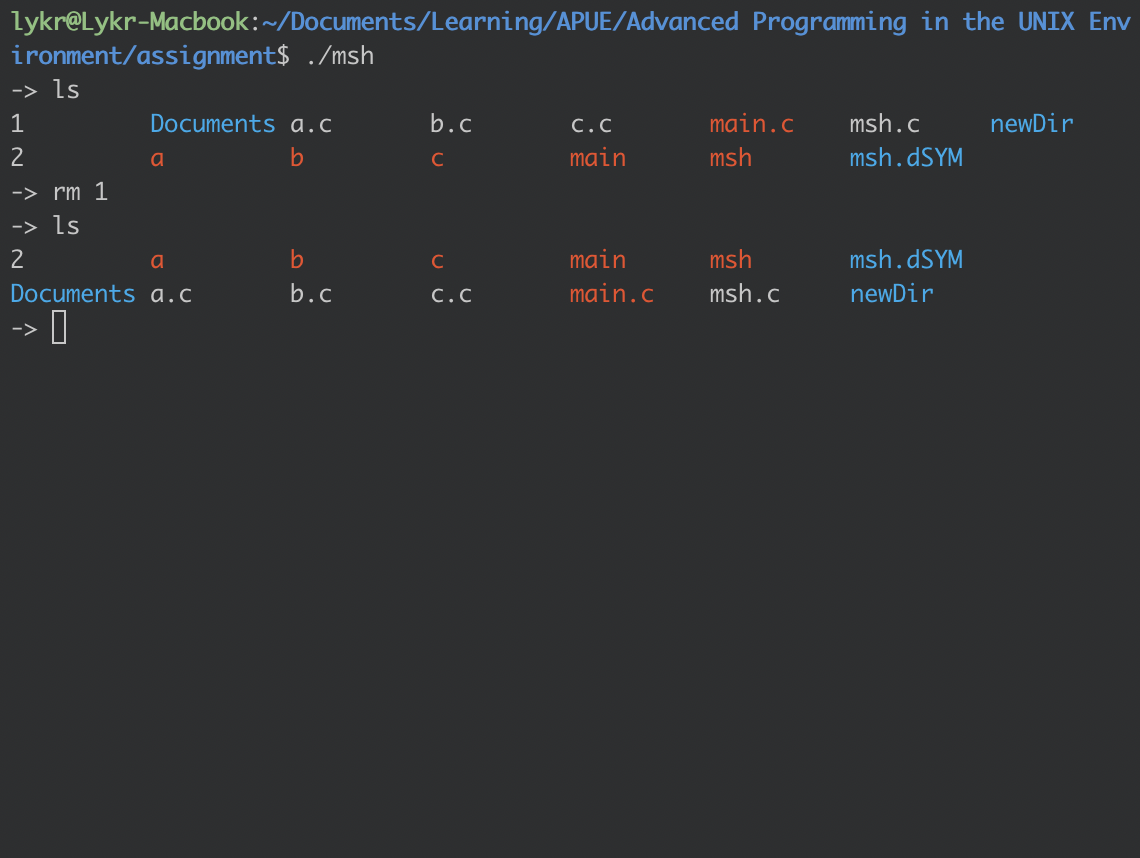
\includegraphics[scale=0.4]{fig/v5-4.png}
\caption{Command `rm'}
\end{figure}

\newpage
\section{DEVELOPMENT ENVIRONMENT}

\begin{itemize}
\item Hardware: Macbook pro 2018
\item System: Mac OS 10.14.4
\item Code Software: Visual Studio Code
\item Compiler: GCC 4.2.1
\end{itemize}

\end{document}